\subsection{Documentação Typedoc}
Durante a implementação do typedoc foi detetado que a categorização de documentação não se encontrava funcional devido a um problema encontrado pelos desenvolvedores da ferramenta. Foi decidido então reduzir a versão para uma com a funcionalidade ativa, mas esta não se encontrava compatível com a versão mais atualizada de \textit{typescript}, pelo que não foi possível explorar esta funcionalidade. Para contornar o problema foi decidido explorar outra funcionalidade menos utilizada, esta permite converter qualquer documentação em módulos, estes podem então ser categorizados, o problema é que é criado um modelo genérico do código o qual não permite a fácil identificação das tipagens de \textit{scripts}. Estes módulos permitem também a categorização dos mesmos, o que permite um nível de organização da documentação gerada maior.

\begin{figure}[htb]
  \centering
  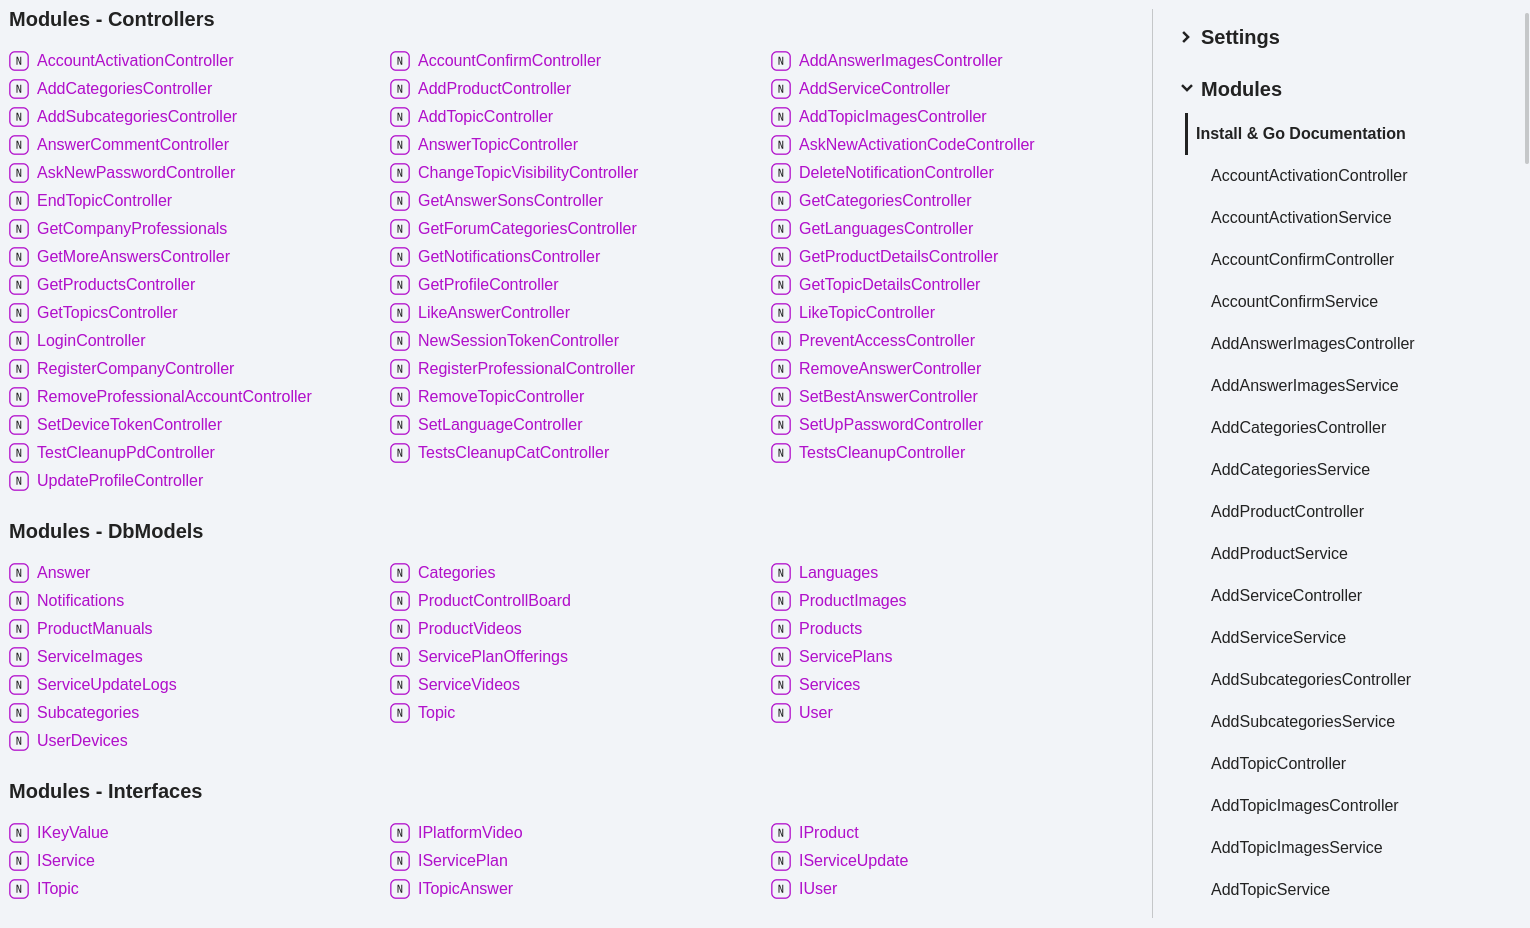
\includegraphics[width=0.8\textwidth]{images/implementacao/api/docs.png}
  \caption{Documentação \textit{typedoc}}
  \label{type_doc}
\end{figure}

\begin{figure}[htb]
  \centering
  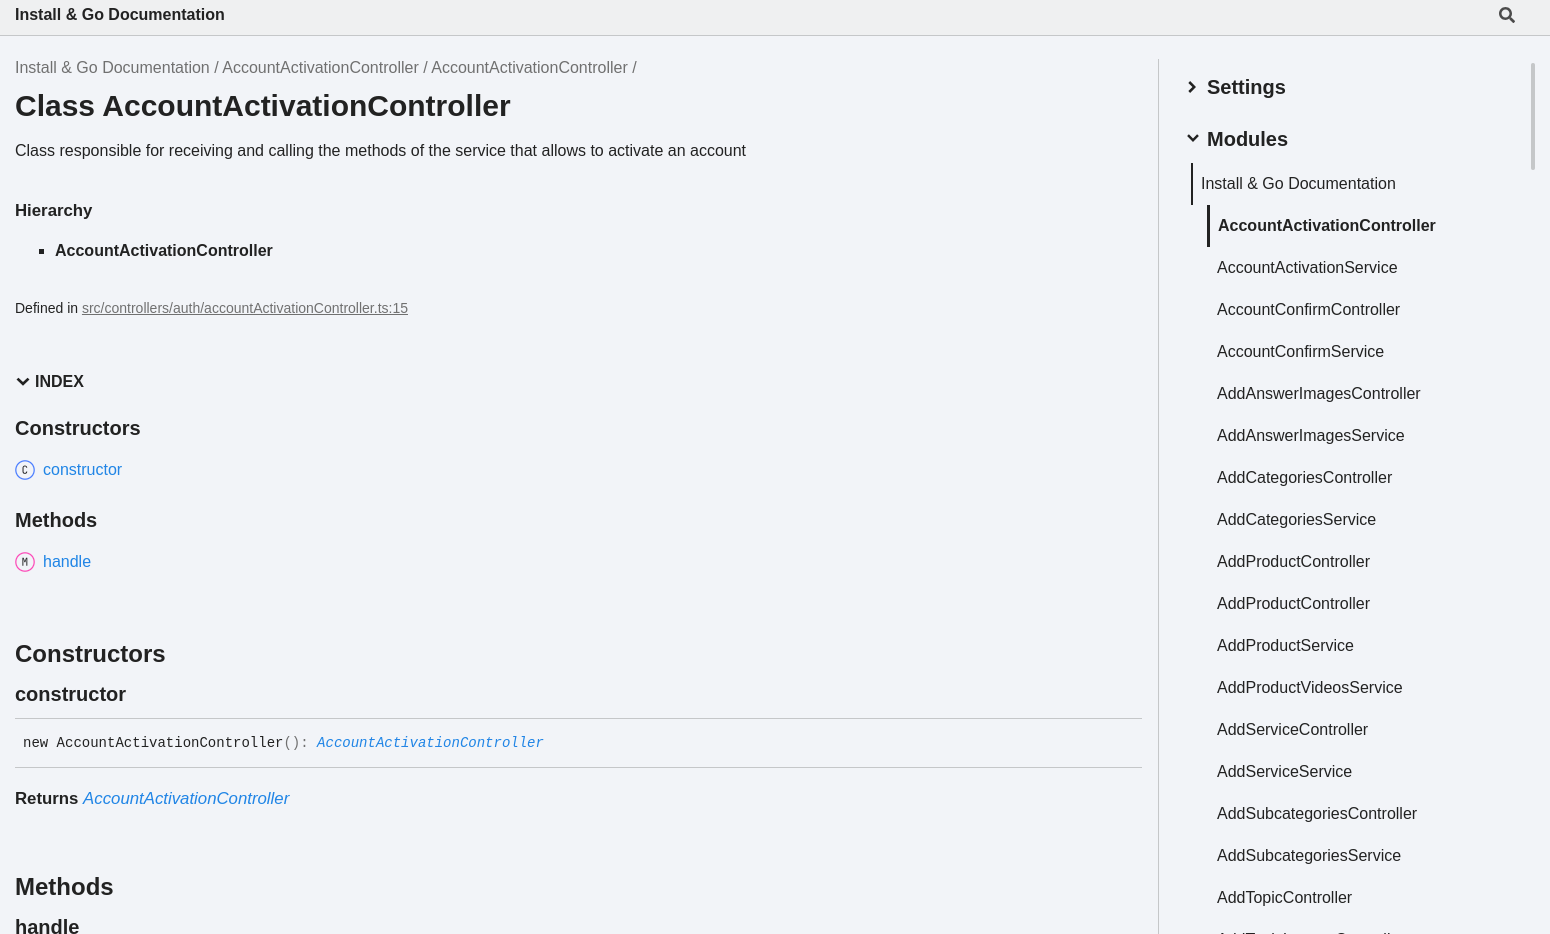
\includegraphics[width=0.8\textwidth]{images/implementacao/api/docs_det.png}
  \caption{Documentação de classe \textit{typedoc}}
  \label{type_doc_det}
\end{figure}

\newpage

\subsection{Documentação Swagger}
Apesar do swagger ferramenta disponibilizar a funcionalidade de gerar automáticamente documentação a partir de comentários de código, foram encontrados alguns problemas com esta funcionalidade, o que levou a que não fosse possível não gerar a documentação. Visto isto, foi optado por manter a documentação manualmente com o ficheiro \textit{json}. Esta ferramenta oferece diversas funcionalidades como autenticação, definição de estruturas de dados para os serviços e exemplos de respostas, ambas estas funcionalidades foram exploradas o que permitiu um bom suporte de documentação para qualquer utilizador.

\begin{figure}[htb]
  \centering
  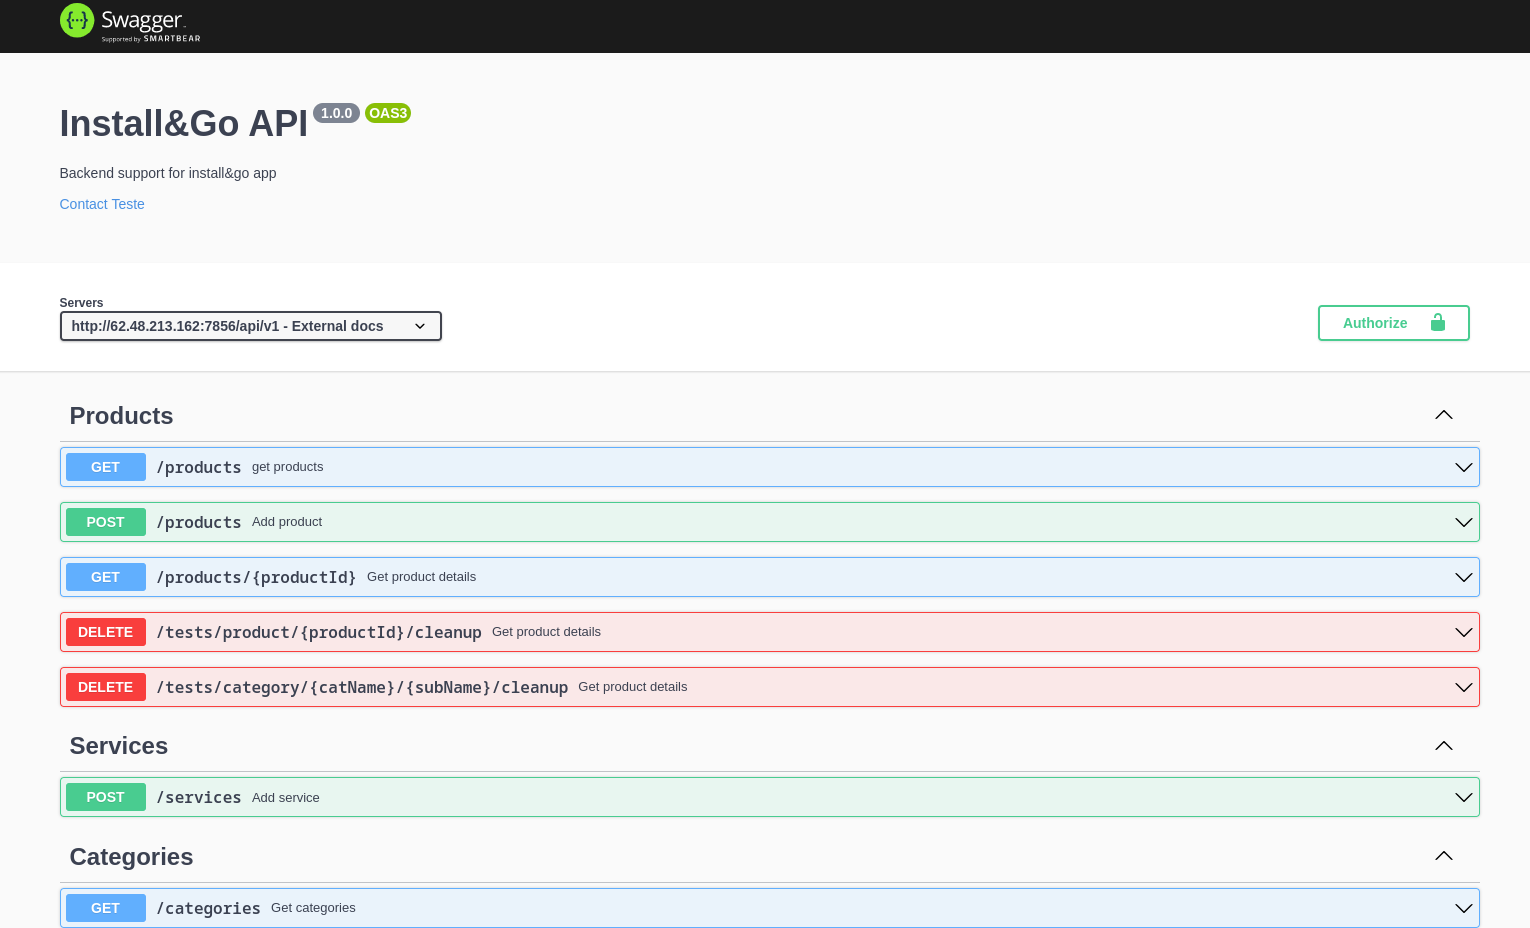
\includegraphics[width=0.7\textwidth]{images/implementacao/api/swagger_intro.png}
  \caption{Documentação swagger}
  \label{fig:67}
\end{figure}

\begin{figure}[htb]
  \centering
  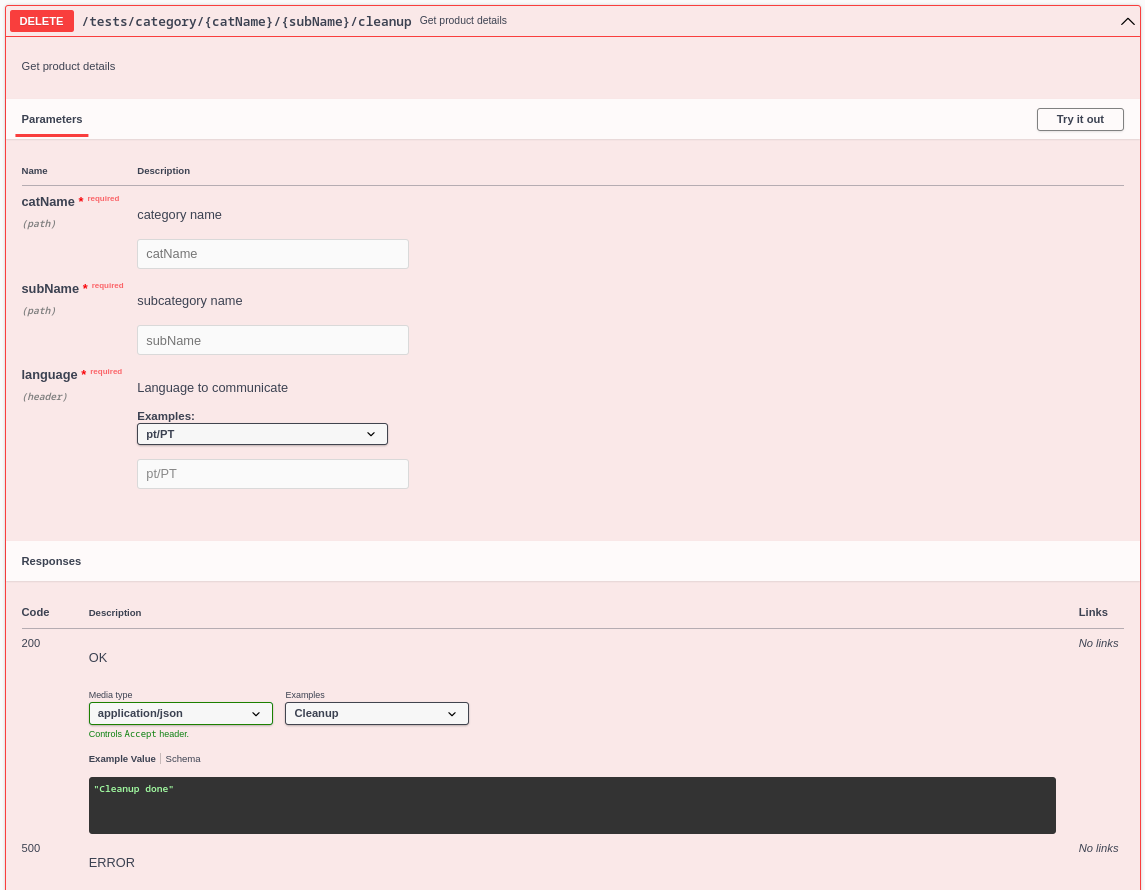
\includegraphics[width=0.7\textwidth]{images/implementacao/api/swagger_pedido.png}
  \caption{Exemplo de documentação de serviço}
  \label{fig:68}
\end{figure}